\documentclass[pdflatex,sn-mathphys-ay]{sn-jnl}

\usepackage{graphicx}
\usepackage{amsmath,amssymb,amsfonts}
\usepackage{amsthm}
\usepackage{booktabs}
\setlength{\bibsep}{0.7em}

\theoremstyle{thmstyleone}
\newtheorem{proposition}{Proposition}

\begin{document}

\title[Defector-Responsive Strategy Switching]{Analytical and Finite-Population Properties of Defector-Responsive Strategy Switching}

\author*[1]{\fnm{Aarush} \sur{Gunjal}}\email{aarushgunjal1@gmail.com}
\affil*[1]{\orgname{Independent Researcher}, \orgaddress{\city{Newark}, \state{Delaware}, \country{USA}}; \href{https://orcid.org/0009-0004-4007-532X}{ORCID: 0009-0004-4007-532X}}

\abstract{
Defector-responsive switching from unconditional cooperation to Tit-for-Tat has been proposed as a rescue mechanism in the repeated Prisoner's Dilemma. The response rule itself was presented by Pal and coauthors; here we characterize analytical and finite-population consequences that were not established there. We derive an exact break-even readiness cost for general benefit and cooperation-cost parameters and state the existence and invasion conditions under which the comparison is valid. We then formulate a continuous-time finite-population process with separate birth-death and individual strategy-transition events. Its infinitesimal drift converges to the deterministic replicator-switching equations, resolving the timescale and interpretation problems created when switching is attached to reproduction. Simulations show that constant switching produces Tit-for-Tat rapidly but continues to remove unconditional cooperators after defectors disappear. Responsive switching can rescue slightly less reliably at low intensity, but it shuts off after rescue and preserves unconditional cooperation over 10 to 100 demographic generations. This preservation advantage remains positive across 27 combinations of population size, selection strength, and benefit-to-cost ratio. Adding the readiness cost to the stochastic process reduces the responsive advantage continuously but does not erase it over the tested finite horizons. The results provide a deterministic-stochastic correspondence, a quantitative cost constraint, and a robust finite-population tradeoff for an existing feedback mechanism.
}

\keywords{evolutionary game theory, repeated Prisoner's Dilemma, state-dependent switching, continuous-time Moran process, cooperation, feedback dynamics}

\maketitle

\section{Introduction}

The Prisoner's Dilemma expresses a conflict between individual and collective benefit: defection is individually favored in a single encounter, although mutual cooperation yields the larger joint return. Repeated interaction can change the evolutionary outcome because strategies may condition present behavior on earlier actions \citep{axelrod1981,axelrod1984,nowak2006}. Tit-for-Tat (TFT), which cooperates initially and then copies its opponent's preceding action, can punish unconditional defection while continuing to cooperate with unconditional cooperators \citep{nowak1992}. The repeated game supports a much broader space of conditional and memory-dependent strategies \citep{stewart2013}.

Evolutionary game dynamics provide a natural framework for asking whether conditional behavior can protect a population dominated by unconditional cooperation. Replicator and selection-mutation equations describe the corresponding infinite-population dynamics \citep{taylor1978,hofbauer1998,hofbauer1985,hadeler1981,page2002}. Mutation can change both the number and stability of equilibria, including in multi-strategy and noisy social dilemmas \citep{antal2009,chen2024}. Finite-population formulations add demographic stochasticity and distinguish invasion, extinction, and fixation events \citep{moran1962,nowak2004,traulsen2006,fudenberg2006}. In repeated games, mutation can reorganize cycles of cooperation and defection or promote diverse cooperative communities \citep{imhof2005,imhof2007,tkadlec2023}.

\citet{pal2025} studied a rescue mechanism with three strategies: unconditional cooperation (ALLC), TFT, and unconditional defection (ALLD). In their principal deterministic model, switching from ALLC to TFT occurs at a constant rate. TFT can suppress an ALLD invasion, but constant switching also continues after the invasion has ended. Pal et al. also considered switching proportional to ALLD abundance in their electronic supplementary material, Figure S8. The feedback rule used here is therefore not claimed as a new mechanism.

Our contribution is to characterize three consequences of that rule. First, we add a payoff cost for maintaining a defector-responsive switching capability. We derive the exact cost at which the cooperative boundary equilibrium matches its constant-switching counterpart for arbitrary benefit $b$ and cooperation cost $c$, together with the stability restrictions required for the comparison. Second, we construct a continuous-time finite-population process whose individual switching events are separate from reproduction and whose large-population drift equals the deterministic equations. This provides a direct deterministic-stochastic correspondence rather than an update-dependent rate-to-probability conversion. Third, we test the resulting tradeoff across post-rescue horizons, population sizes, selection strengths, benefit-to-cost ratios, and readiness costs.

This state-dependent transition belongs to a broader class of feedback in evolutionary dynamics. State-dependent mutation can alter long-run selection \citep{bergin1996}; game-environment feedback can make strategies and environmental states coevolve \citep{weitz2016}; and perception of social information can enter evolutionary decision rules directly \citep{salahshour2025}. The present model is narrower: the current ALLD frequency changes the transition intensity between two fixed strategies, not the payoff matrix or the perceived action itself.

\section{Model}

\subsection{Repeated-game payoffs}

Let $x$, $y$, and $z$ be the frequencies of ALLC, TFT, and ALLD, respectively, with $x+y+z=1$. We use the payoff convention of \citet{pal2025}:
\begin{equation}
\label{eq:matrix}
\begin{array}{c|ccc}
 & \mathrm{ALLC} & \mathrm{TFT} & \mathrm{ALLD}\\ \hline
\mathrm{ALLC} & b-c & b-c & -c\\
\mathrm{TFT}  & b-c & (b-c)/2 & 0\\
\mathrm{ALLD} & b   & 0       & 0
\end{array}.
\end{equation}
This matrix comes from an infinitely repeated donation game in the limit of rare implementation error. An intended cooperation is implemented as defection with probability $\alpha\epsilon$, and an intended defection is implemented as cooperation with probability $\beta\epsilon$. Payoffs are long-run averages under the stationary distribution of the four outcomes $CC$, $CD$, $DC$, and $DD$, followed by the limit $\epsilon\to0^+$. Pal et al. take symmetric errors, $\alpha=\beta$. In a TFT-TFT match the four outcomes then have equal limiting stationary weight, giving
\begin{equation}
\frac{(b-c)+(-c)+b+0}{4}=\frac{b-c}{2}.
\end{equation}
Thus, the TFT-TFT entry is not the noiseless value. Without implementation error, mutual TFT beginning with cooperation would instead receive $b-c$ per round.

Writing $q=b-c>0$, the expected payoffs are
\begin{align}
f_C &= q(x+y)-cz, &
f_T &= q(x+y/2), &
f_D &= bx, \label{eq:payoffs}
\end{align}
and $\bar f=xf_C+yf_T+zf_D$.

\subsection{Deterministic switching dynamics}

One-way switching from ALLC to TFT gives
\begin{align}
\dot x &=x(f_C-\bar f)-\mu x,\nonumber\\
\dot y &=y(f_T-\bar f)+\mu x,\label{eq:replicator}\\
\dot z &=z(f_D-\bar f).\nonumber
\end{align}
We compare a constant rule, $\mu=\mu_0$, with the defector-responsive rule, $\mu=\mu_0z$.

To represent the cost of maintaining the responsive capability, the payoff of ALLC is reduced by $k\geq0$. Thus, $f_C$ is replaced by $f_C-k$ in its replicator term and the population mean becomes $\bar f_k=\bar f-kx$. The switching flow remains $\mu_0zx$. The cost is state-specific: it represents maintaining the latent ALLC program in readiness to detect defectors and enter the TFT phenotype. After an individual switches, it has left that latent state and no longer pays this particular readiness cost. A persistent sensing cost paid by both ALLC and TFT would be a different model and would remove the interior ALLC-TFT boundary balance derived below.

\subsection{Continuous-time finite-population process}

The finite model is a continuous-time Moran-type birth-death process with a separate phenotypic transition channel. Let $\boldsymbol n=(n_C,n_T,n_D)$, $N=n_C+n_T+n_D$, and $\boldsymbol X^N=\boldsymbol n/N$. Expected payoffs $\pi_i^N$ are calculated against the other $N-1$ individuals using \eqref{eq:matrix}. In the responsive costly model, $k$ is subtracted from $\pi_C^N$ only. An individual of type $i$ gives birth at rate
\begin{equation}
r_i=a+w\pi_i^N,\qquad a=3,
\label{eq:birthrate}
\end{equation}
and its offspring replaces a uniformly selected individual. The common baseline $a$ keeps all birth rates nonnegative over the reported parameter ranges and cancels from the deterministic selection drift. The parameter $w$ controls selection strength.

Independently of reproduction, each ALLC individual changes phenotype to TFT at intensity $\mu_0$ under constant switching and $\mu_0n_D/N$ under responsive switching. The corresponding population-level transition rates are
\begin{equation}
q_{C\to T}^{N}=\mu_0n_C
\quad\text{and}\quad
q_{C\to T}^{N}=\mu_0\frac{n_D}{N}n_C,
\label{eq:switchrates}
\end{equation}
respectively. A transition changes an existing individual, rather than the type of a newborn. Consequently, it represents behavioral or phenotypic switching, not mutation or transmission error.

\begin{proposition}[Deterministic limit]
Let $h(z)=1$ for constant switching and $h(z)=z$ for responsive switching. For a smooth test function $\varphi$, the generator of the frequency process is
\begin{align}
\mathcal L_N\varphi(\boldsymbol x)
={}&N\sum_{i,j}x_ix_jr_i
\left[\varphi\!\left(\boldsymbol x+\frac{\boldsymbol e_i-\boldsymbol e_j}{N}\right)-\varphi(\boldsymbol x)\right]\nonumber\\
&+N\mu_0xh(z)
\left[\varphi\!\left(\boldsymbol x+\frac{\boldsymbol e_T-\boldsymbol e_C}{N}\right)-\varphi(\boldsymbol x)\right].
\label{eq:generator}
\end{align}
Its infinitesimal drift converges as $N\to\infty$ to
\begin{equation}
w\begin{pmatrix}
x(\widetilde f_C-\overline{\widetilde f})\\
y(f_T-\overline{\widetilde f})\\
z(f_D-\overline{\widetilde f})
\end{pmatrix}
+\mu_0xh(z)
\begin{pmatrix}-1\\1\\0\end{pmatrix},
\label{eq:drift}
\end{equation}
where $\widetilde f_C=f_C-k$ in the costly responsive model, $\widetilde f_C=f_C$ otherwise, and $\overline{\widetilde f}=x\widetilde f_C+yf_T+zf_D$. For $w=1$, \eqref{eq:drift} is exactly \eqref{eq:replicator}, including its switching flux.
\end{proposition}

\noindent\emph{Proof.}
For coordinate $i$, a birth-death event contributes
\begin{equation}
\sum_j x_ix_j(r_i-r_j)
=x_i(r_i-\bar r)
=wx_i(\widetilde f_i-\overline{\widetilde f}),
\end{equation}
because the common baseline $a$ cancels. The transition in \eqref{eq:switchrates} contributes $\mu_0xh(z)(-1,1,0)^\mathsf T$. Finite-population payoffs calculated without self-interaction converge uniformly to \eqref{eq:payoffs}. Standard fluid-limit results for density-dependent jump processes then give convergence on finite time intervals under the usual regularity conditions \citep{kurtz1970}. \hfill$\square$

This construction fixes the time unit explicitly: payoffs determine individual birth rates through \eqref{eq:birthrate}, while $\mu_0$ is an individual transition intensity in the same continuous-time clock. No unit-length interval is inserted into a probability transformation.

\section{Analytical Cost Result}

The boundary $z=0$ permits a direct comparison of the two switching rules. It is also where their difference is clearest: constant switching remains active, whereas defector-responsive switching stops.

\begin{proposition}[Break-even readiness cost]
Assume $b>c>0$ and write $q=b-c$.
\begin{enumerate}
\item Under constant switching, the nontrivial ALLC-TFT boundary equilibrium is
\begin{equation}
x_F^*=1-\sqrt{\frac{2\mu_0}{q}},\qquad
y_F^*=\sqrt{\frac{2\mu_0}{q}},
\label{eq:fixededge}
\end{equation}
and exists for $0\leq\mu_0\leq q/2$. Its transverse ALLD invasion exponent is
\begin{equation}
g_F(\mu_0)=c-b\sqrt{\frac{2\mu_0}{q}}+\mu_0.
\label{eq:fixedinv}
\end{equation}
\item Under defector-responsive switching with readiness cost $k$, the nontrivial boundary equilibrium is
\begin{equation}
x_R^*=1-\frac{2k}{q},\qquad y_R^*=\frac{2k}{q},
\label{eq:adaptiveedge}
\end{equation}
and exists for $0\leq k\leq q/2$. It resists an infinitesimal ALLD invasion if
\begin{equation}
k>\frac{cq}{b+c}.
\label{eq:adaptiveinv}
\end{equation}
\item Whenever the two boundary equilibria are the relevant stable outcomes, their ALLC frequencies are equal at
\begin{equation}
k^*(\mu_0)=\sqrt{\frac{q\mu_0}{2}}.
\label{eq:threshold}
\end{equation}
For $cq/(b+c)<k<k^*(\mu_0)$, the responsive equilibrium contains more ALLC than the constant-switching equilibrium.
\end{enumerate}
\end{proposition}

\noindent\emph{Proof.}
On $z=0$, let $y=1-x$. For constant switching, the ALLC equation reduces to
\begin{equation}
\dot x=x\left(\frac{q}{2}y^2-\mu_0\right),
\end{equation}
which gives \eqref{eq:fixededge}. At that equilibrium the mean payoff is $q-\mu_0$, so the growth rate of rare ALLD is $b(1-y_F^*)-(q-\mu_0)$, yielding \eqref{eq:fixedinv}.

For responsive switching, $\mu_0z=0$ on the boundary. Coexistence requires equality of the cost-adjusted ALLC and TFT payoffs: $q-k=q(1-y/2)$. This gives \eqref{eq:adaptiveedge}. The growth rate of rare ALLD is
\begin{equation}
b\left(1-\frac{2k}{q}\right)-(q-k)
=c-\frac{b+c}{q}k,
\end{equation}
which is negative precisely under \eqref{eq:adaptiveinv}. Finally, equating \eqref{eq:fixededge} and \eqref{eq:adaptiveedge} gives \eqref{eq:threshold}; the strict comparison follows from the same expressions. \hfill$\square$

For $b=5$ and $c=1$, \eqref{eq:threshold} becomes $k^*=\sqrt{2\mu_0}$, while transverse stability of the responsive boundary requires $k>2/3$. At the break-even value this condition holds when $\mu_0>2/9$. The constant boundary is transversely stable when $g_F(\mu_0)<0$ and exists through $\mu_0=2$.

\section{Numerical Methods}

The deterministic system was integrated from $(x,y,z)=(1/3,1/3,1/3)$ to $t=800$ with an eighth-order adaptive solver, relative tolerance $2\times10^{-11}$, and absolute tolerance $2\times10^{-13}$. The implementation neither clips negative values nor renormalizes the state after integration; terminal states were checked against the simplex constraint.

The continuous-time jump process was simulated exactly by sampling the next event from the total birth and switching rates. Each trial began with $N-1$ ALLC individuals and one ALLD individual. Rescue occurred when ALLD first reached extinction, failure occurred when ALLD fixed, and pre-rescue observation was capped after $1000N$ birth-death events. No reported trial was censored. After rescue, composition was recorded after $10N,20N,\ldots,100N$ additional birth-death events; switch events occurring between those events remained part of the continuous-time process.

The main sweep used $N=100$, $b=5$, $c=1$, $w=1$, 11 values of $\mu_0$ from 0 to 2, and 500 independent trials per point. Robustness was evaluated at $\mu_0=1$ for all 27 combinations of $N\in\{50,100,200\}$, $w\in\{0.25,0.5,1\}$, and $b/c\in\{3,5,7\}$ with $c=1$ and 300 trials per combination. The cost sweep used $N=100$, $b=5$, $c=1$, $w=1$, $\mu_0=1$, $k\in\{0,0.2,\ldots,2\}$, and 400 trials per nonzero cost. Means are shown with normal-approximation 95\% confidence intervals. Source code, fixed random seeds, and numerical output are provided in the repository.

\section{Results}

\subsection{Deterministic comparison and cost threshold}

Figure \ref{fig:deterministic}A shows that constant switching progressively removes ALLC as $\mu_0$ increases, while responsive switching rises to a high-ALLC equilibrium over the plotted range. At $\mu_0=0.5$, the terminal ALLC frequencies are $0.500$ under constant switching and $0.643$ under responsive switching; at $\mu_0=1$, they are $0.293$ and $0.701$, respectively. At $\mu_0=2$, the constant-switching boundary reaches zero ALLC, while the responsive trajectory has terminal ALLC frequency $0.738$.

For the costly model, we evaluated \eqref{eq:threshold} at 31 values of $\mu_0$ from $0.45$ to $1.95$. Figure \ref{fig:deterministic}B displays the predicted curve. The maximum absolute difference between the numerically integrated costly-responsive ALLC equilibrium and its constant-switching counterpart was $2.28\times10^{-11}$. This check supports the implementation, while the threshold itself follows analytically from the proposition.

\begin{figure}[htbp]
\centering
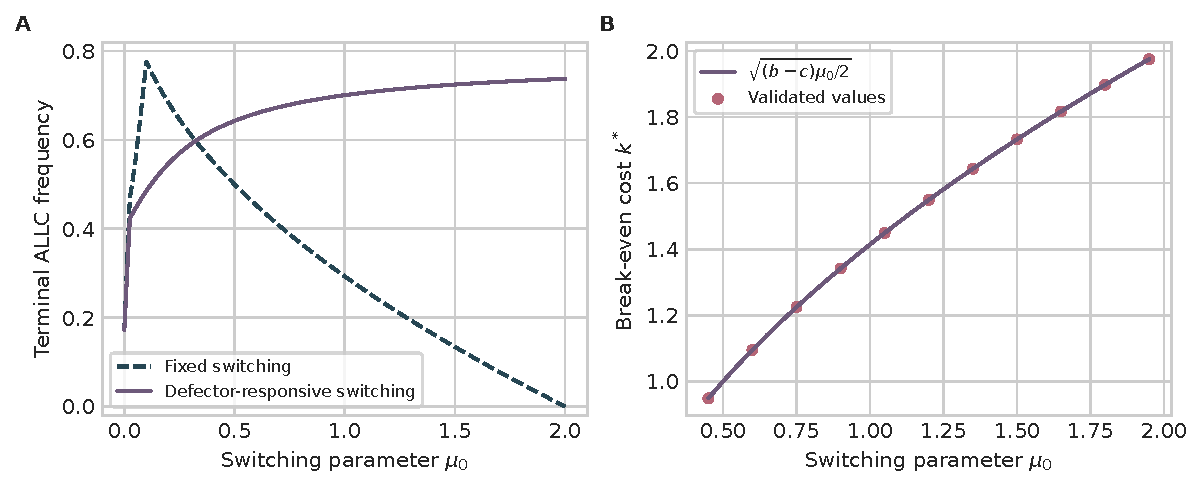
\includegraphics[width=\textwidth]{Fig1.pdf}
\caption{Deterministic comparison for $b=5$ and $c=1$. (A) Terminal ALLC frequency from an interior initial condition under constant and defector-responsive switching. (B) Exact break-even readiness cost from \eqref{eq:threshold}; markers show parameters checked by numerical integration.}
\label{fig:deterministic}
\end{figure}

\subsection{Finite-population tradeoff and post-rescue horizon}

Figure \ref{fig:finite} separates rescue probability, composition at rescue, and composition over time after rescue. At low intensity, constant switching rescues more reliably because it creates TFT without waiting for a strong defector signal. At $\mu_0=0.2$, rescue probabilities are $0.996$ for constant switching and $0.930\pm0.022$ for responsive switching. By $\mu_0=1$, both are near one: $1.000$ and $0.996\pm0.006$.

The post-rescue comparison reverses. At $\mu_0=1$, the mean ALLC frequencies at rescue are $0.787\pm0.008$ and $0.935\pm0.005$ for constant and responsive switching. After $10N$ additional birth-death events they are $0.355\pm0.013$ and $0.960\pm0.009$; after $50N$, $0.187\pm0.015$ and $0.985\pm0.007$; and after $100N$, $0.121\pm0.014$ and $0.988\pm0.007$. Constant switching continues to convert ALLC to TFT after $z=0$. Responsive switching stops immediately, after which selection and drift on the ALLC-TFT edge generally restore ALLC. The time course therefore reflects a structural difference, not a transient created by selecting a single horizon.

\begin{figure}[htbp]
\centering
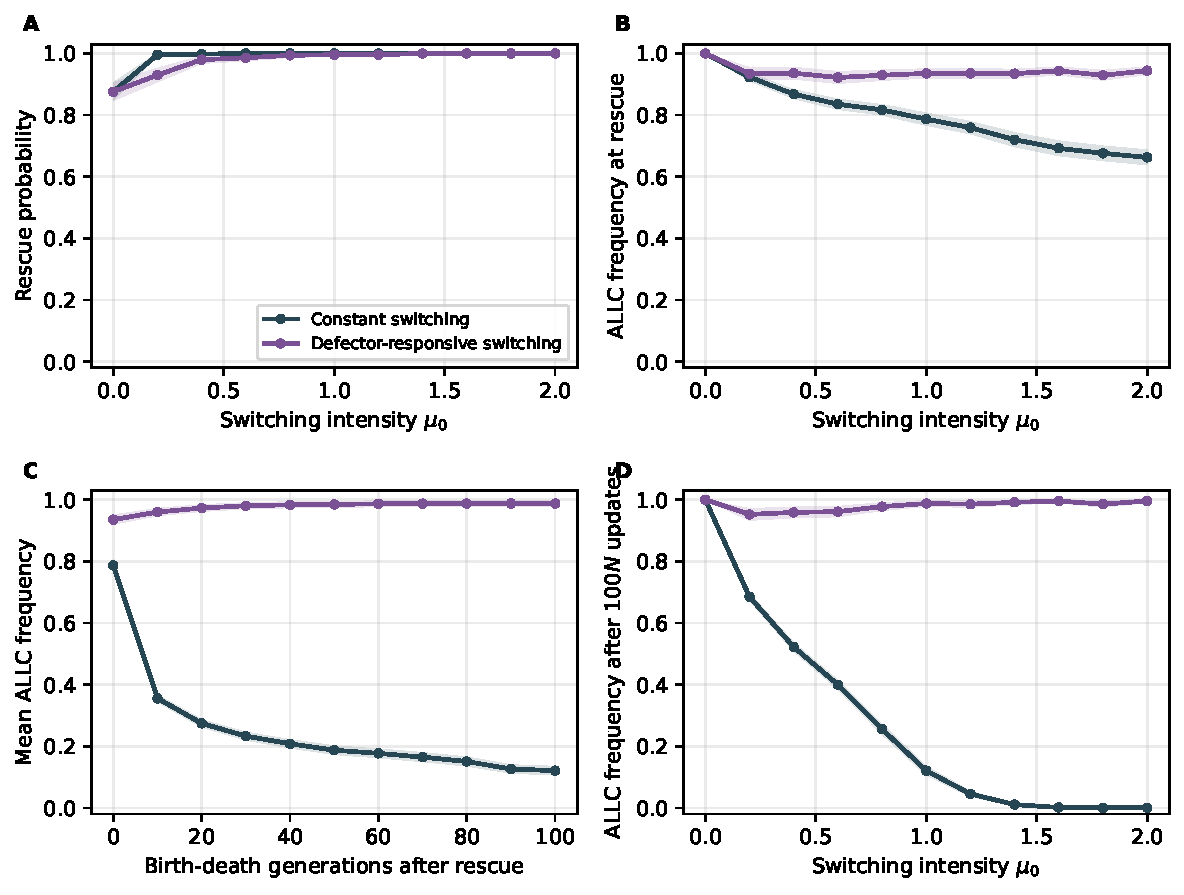
\includegraphics[width=\textwidth]{Fig2_revised.pdf}
\caption{Continuous-time finite-population results for $N=100$, $b=5$, $c=1$, $w=1$, and 500 trials per point. Lines show means and shading shows 95\% confidence intervals. (A) Probability that ALLD reaches extinction before fixation. (B) ALLC frequency at first ALLD extinction. (C) Post-rescue time course at $\mu_0=1$. One demographic generation is $N$ birth-death events. (D) ALLC frequency after $100N$ post-rescue birth-death events.}
\label{fig:finite}
\end{figure}

\subsection{Robustness and readiness cost}

The preservation advantage survives all requested parameter changes (Figure \ref{fig:robustness}A). Across the 27 combinations of $N$, $w$, and $b/c$, the responsive-minus-constant difference in mean ALLC frequency after $100N$ post-rescue birth-death events ranges from $0.594$ to $0.999$. This advantage is not produced by a large rescue-probability benefit. Responsive switching has a rescue probability between 0 and 0.040 below the constant rule across the same combinations (Figure \ref{fig:robustness}B). Thus, the robust tradeoff is slightly weaker or equal rescue paired with substantially better post-rescue preservation.

Including $k$ in the finite process connects the stochastic comparison to the analytical result. At $\mu_0=1$, the deterministic break-even value is $k^*=\sqrt{2}\approx1.414$. As $k$ rises from 0 to 2, responsive rescue probability remains between $0.980$ and $1.000$, but its mean ALLC frequency after $100N$ events falls from $0.988$ at $k=0$ to $0.658$ at $k=1.4$ and $0.575$ at $k=2$ (Figure \ref{fig:robustness}C,D). The cost-free constant benchmark is $0.121$ at the same horizon. The deterministic threshold is not expected to be an exact crossing point for this conditional finite-time statistic, but it correctly identifies the parameter scale on which readiness cost materially erodes the responsive advantage.

\begin{figure}[htbp]
\centering
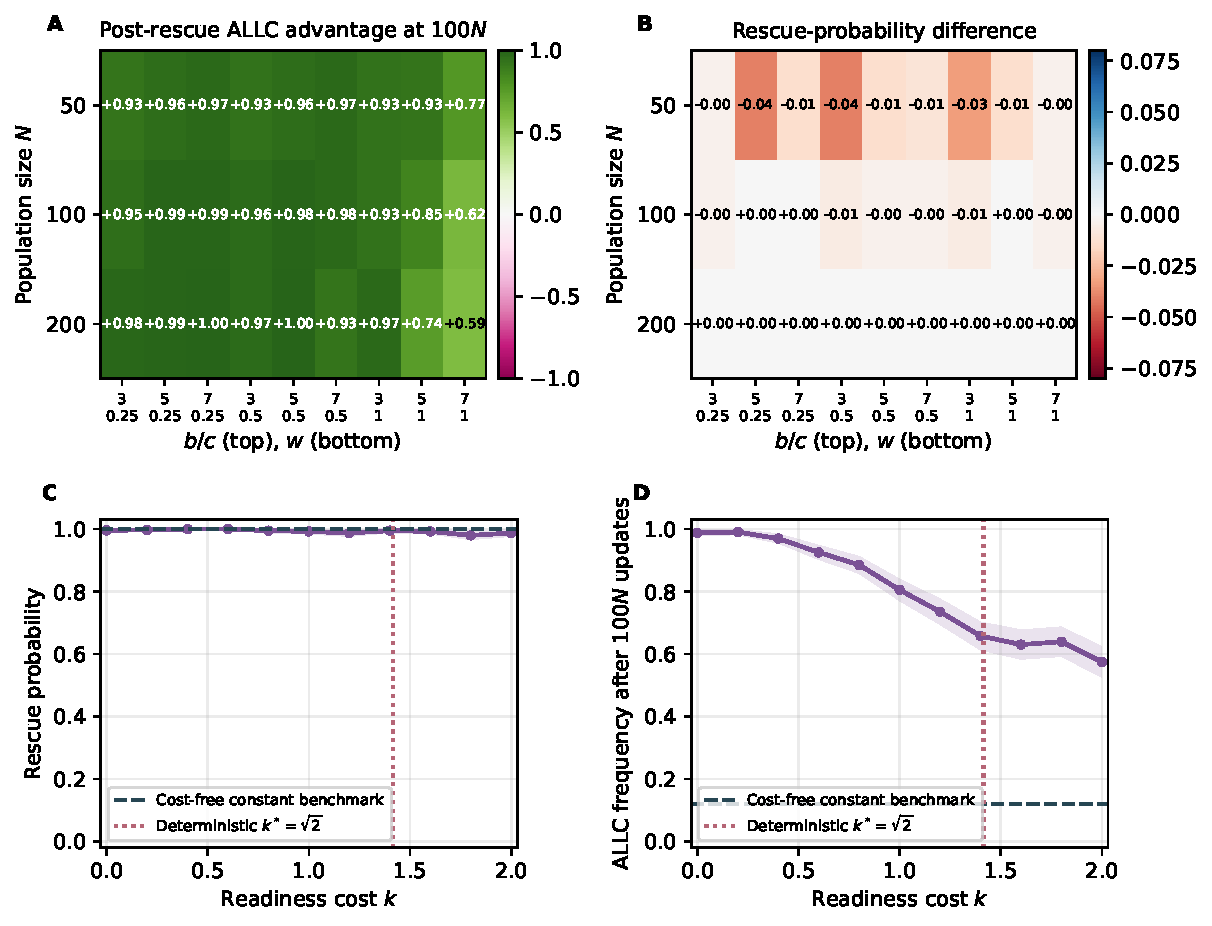
\includegraphics[width=\textwidth]{Fig3_revised.pdf}
\caption{Robustness and readiness cost. (A,B) Responsive-minus-constant differences at $\mu_0=1$ across 27 combinations of population size, selection strength, and benefit-to-cost ratio; values are based on 300 trials per condition. (A) ALLC frequency after $100N$ post-rescue birth-death events. (B) Rescue probability. (C,D) Cost sweep for the responsive process with 400 trials per nonzero cost. Dashed lines show the cost-free constant benchmark and dotted lines show the deterministic threshold $k^*=\sqrt{2}$. (C) Rescue probability. (D) ALLC frequency after $100N$ events.}
\label{fig:robustness}
\end{figure}

\section{Discussion}

The defector-proportional response is an appealing negative-feedback mechanism, but it is not new to this paper: \citet{pal2025} presented it in Supplementary Figure S8. The present study adds a general cost theorem with stability restrictions, a continuous-time individual process with a derived deterministic limit, and a robustness analysis across demographic and game parameters. These additions convert the finite-population comparison from a reproduction-linked mutation rule into a model of individual phenotype change and clarify which conclusions depend on time horizon.

The distinction from earlier finite-population work is important. \citet{imhof2007} studied mutation-selection dynamics among ALLC, ALLD, and TFT and emphasized the vulnerability of TFT to drift toward ALLC. Here, transition is one-way and activated by current ALLD abundance; the question is not which strategy dominates under recurrent mutation, but how a temporary responsive phenotype can rescue and then preserve an ALLC population. Likewise, game-environment feedback changes payoffs as an environmental state evolves \citep{weitz2016}, whereas the present feedback changes only the ALLC-to-TFT transition intensity. The information assumption is closer to perceptual evolutionary models in which decisions depend on social or environmental signals \citep{salahshour2025}, although our signal is the exact global frequency $z$.

The post-rescue horizon cannot be omitted. Once ALLD disappears, responsive switching stops but constant one-way switching continues. In a finite population, the long-run absorbing structures therefore differ: responsive dynamics on the ALLC-TFT edge ultimately reaches one of its monomorphic endpoints, while constant switching makes all-ALLC nonabsorbing and favors eventual loss of ALLC. Results at $10N$, $50N$, and $100N$ show how this structural difference emerges rather than presenting a single selected endpoint.

The readiness cost is intentionally specific. It represents the opportunity or maintenance cost of remaining in an ALLC state that is prepared to detect defectors and activate TFT. If a biological system instead pays a persistent sensing cost after activation, both the payoff model and the boundary theorem must change. The stochastic cost sweep shows that the state-specific cost can strongly reduce post-rescue ALLC even when rescue remains likely, so cost cannot be ignored when evaluating the mechanism.

Several limitations remain. The response uses instantaneous global knowledge of $z$; local, delayed, or noisy perception could change activation. The payoff matrix is a reduced limit of an infinitely repeated donation game with symmetric rare implementation errors, not the standard noiseless repeated Prisoner's Dilemma. The common birth-rate baseline $a$ affects demographic event speed and finite-population variance even though it cancels from deterministic drift. Finally, the model contains only one switching direction. A biologically specific application would require a mechanistic sensing timescale, local information, a persistent-cost decision, and parameters tied to data.

\section{Conclusion}

Defector-responsive switching trades slightly weaker rescue at low signal strength for substantially better preservation of unconditional cooperation after rescue. The exact deterministic break-even cost is $k^*(\mu_0)=\sqrt{(b-c)\mu_0/2}$ subject to explicit existence and invasion conditions. A continuous-time Moran-type process with separate individual transitions converges directly to the deterministic equations and gives the switching intensity an unambiguous timescale and phenotype interpretation. The resulting finite-population tradeoff persists across population size, selection strength, benefit-to-cost ratio, post-rescue horizon, and readiness cost.

\backmatter

\section*{Acknowledgements}

The author thanks Dr. Saptarshi Pal for expert advice and helpful discussions concerning the evolutionary-game model.

\section*{Statements and Declarations}

\subsection*{Funding}

No funds, grants, or other support were received.

\subsection*{Competing Interests}

The author has no relevant financial or non-financial interests to disclose.

\subsection*{Author Contributions}

Aarush Gunjal performed the conceptualization, methodology, formal analysis, software development, numerical investigation, visualization, and manuscript preparation. The author read and approved the final manuscript.

\subsection*{Data Availability}

The numerical data supporting the findings of this study are available in the public repository at \url{https://github.com/aarushgunjal/defector_responsive_strategy_switching}.

\subsection*{Code Availability}

The source code and figure-generation materials needed to reproduce the reported results are available at \url{https://github.com/aarushgunjal/defector_responsive_strategy_switching}.

\subsection*{Use of Generative AI}

Generative AI tools were used for language and presentation assistance during manuscript preparation. The author independently reviewed and verified the mathematical analysis, code, citations, numerical results, and final text and accepts full responsibility for the manuscript.

\bibliography{references}

\end{document}
